\chapter{LİTERATÜR, KURAMSAL TEMEL VE ARAŞTIRMA BOŞLUĞU}
\label{chap:literatur}

Giriş bölümünde tezin iki odak noktası tanımlanmıştı: düşük güçteki verim--harmonik ödünleşimi ve aynı T-tipi donanımın enerji depolama işlevlerinde yeniden kullanılması. Literatür bölümü, iki odak noktasını taşıyan dört bilgi alanını inceleyerek araştırma boşluğunu belirlemektedir. Ele alınan dört alan enerji depolama sistemlerinde güç dönüşüm mimarileri, üç seviyeli T-tipi dönüştürücünün kuramsal temeli, fotovoltaik çalışma profili ile kısmi yük performansı ve şebeke akım kontrolündeki ileri besleme yaklaşımlarıdır.

\section{Enerji Depolama Sistemlerinde Güç Dönüşüm Mimarileri}

Enerji depolama sistemleri, elektrik enerjisinin farklı zaman ölçeklerinde depolanmasını ve yeniden kullanılmasını sağlayan çok bileşenli yapılardır. Elektrokimyasal depolamanın yaygınlaşmasıyla birlikte batarya grubu, güç dönüşüm sistemi, batarya yönetim sistemi (Battery Management System, BYS), enerji yönetim sistemi, koruma ve ısıl yönetim birimleri aynı sistem sınırı içinde değerlendirilmeye başlanmıştır \citep{Chen2009,Aneke2016,Hannan2017}. Bileşenlerden güç dönüşüm sistemi, bataryanın değişken doğru gerilimi ile şebeke veya yük arasındaki çift yönlü enerji akışını düzenlemektedir. BYS ise hücre gerilimlerini, sıcaklıkları ve şarj durumunu izleyerek güvenli çalışma sınırlarını korumaktadır \citep{Plett2015,Khan2024}. Her iki işlev fiziksel olarak ayrı birimlerde gerçekleştirilse bile enerji akışı, güvenlik ve kullanılabilir kapasite bakımından birbirine bağımlıdır.

Bileşenler arasındaki güç ve bilgi akışları, tipik bir şebeke bağlantılı EDS için Şekil~\ref{fig:eds-mimarisi} üzerinde özetlenmiştir. Şekilde kesintisiz çizgiler güç aktarım yolunu, kesikli çizgiler ise ölçüm ve yönetim bağlantılarını göstermektedir.

\begin{figure}[H]
  \centering
  \resizebox{0.98\textwidth}{!}{%
  \begin{tikzpicture}[
    node distance=7mm and 7mm,
    guc/.style={draw, rounded corners=1.5pt, align=center, font=\small, minimum height=14mm, text width=27mm, fill=blue!5},
    yon/.style={draw, rounded corners=1.5pt, align=center, font=\small, minimum height=12mm, text width=34mm, fill=orange!10},
    alt/.style={draw, rounded corners=1.5pt, align=center, font=\small, minimum height=11mm, text width=24mm, fill=gray!10},
    akis/.style={-{Latex[length=2mm]}, thick},
    bilgi/.style={{Latex[length=1.6mm]}-{Latex[length=1.6mm]}, dashed}
  ]
    \node[guc] (bat) {Enerji depolama\\elemanı\\(batarya)};
    \node[guc, right=of bat] (da) {DA bara};
    \node[guc, right=of da] (cev) {Çift yönlü güç\\dönüştürücüsü\\(AA/DA)};
    \node[guc, right=of cev] (fil) {LCL filtre};
    \node[guc, right=of fil] (seb) {Şebeke / yük};
    \draw[{Latex[length=2mm]}-{Latex[length=2mm]}, thick] (bat) -- (da);
    \draw[{Latex[length=2mm]}-{Latex[length=2mm]}, thick] (da) -- (cev);
    \draw[{Latex[length=2mm]}-{Latex[length=2mm]}, thick] (cev) -- (fil);
    \draw[{Latex[length=2mm]}-{Latex[length=2mm]}, thick] (fil) -- (seb);
    \node[yon, below=14mm of cev] (eys) {Denetim ve yönetim\\sistemi (EYS / BYS)};
    \draw[bilgi] (bat.south) |- ([yshift=-3mm]eys.west);
    \draw[bilgi] (da.south) |- ([yshift=3mm]eys.west);
    \draw[bilgi] (cev.south) -- (eys.north);
    \draw[bilgi] (seb.south) |- (eys.east);
    \node[alt, below=16mm of eys, xshift=-46mm] (olc) {Ölçüm ve\\izleme sistemi};
    \node[alt, right=of olc] (isi) {Isıl yönetim\\sistemi};
    \node[alt, right=of isi] (yrd) {Yardımcı güç\\kaynakları};
    \node[alt, right=of yrd] (kor) {Koruma ve\\güvenlik sistemi};
    \coordinate (dal) at ([yshift=-7mm]eys.south);
    \draw[dashed] (eys.south) -- (dal);
    \foreach \n in {olc,isi,yrd,kor} {\draw[dashed, -{Latex[length=1.6mm]}] (dal) -| (\n.north);}
  \end{tikzpicture}%
  }
  \caption{Şebeke bağlantılı bir enerji depolama sisteminin temel bileşenleri ve bilgi akışları.}
  \label{fig:eds-mimarisi}
\end{figure}

Geleneksel şebeke bağlantılı bir EDS'de batarya ile DA bara arasında çift yönlü bir DA/DA dönüştürücü, DA bara ile şebeke arasında bir evirici/doğrultucu ve hücreler arasında ayrı bir dengeleme devresi bulunabilir. Katların ayrılması her işlev için bağımsız tasarım ve koruma olanağı sunsa da yarı iletken, manyetik eleman, sürücü, algılayıcı ve soğutma gereksinimini de artırmaktadır. Sistem maliyeti çalışmalarında batarya paketi baskın kalem olmakla birlikte, güç elektroniği donanımının maliyet, kayıp ve hacim üzerindeki etkisi ihmal edilemez \citep{Ramasamy2023,Lazard2024}. İşlevlerin ortak elemanlarla gerçekleştirilmesi, özellikle şarj ve deşarj kiplerinin aynı anda etkin olmadığı uygulamalarda donanım kullanım oranını yükseltme potansiyeli taşımaktadır.

Ortak eleman kullanımının en olgun örneği elektrikli araçlardaki tümleşik şarj cihazlarıdır. \citet{Haghbin2013}, araç şebekeden şarj edilirken çekiş sürücüsü elemanlarının boşta kaldığını ve aynı elemanların yerleşik şarj devresinde kullanılabildiğini belirtmiştir. Aynı çalışmada yalıtımlı ve yalıtımsız tümleşik şarj çözümleri sınıflandırılmış, ayrıca bölünmüş fazlı sürekli mıknatıslı motor sargılarını kullanan, çift yönlü ve birim güç faktörlü, yalıtımlı bir üç fazlı şarj cihazı önerilmiştir. \citet{Yilmaz2013} ise şarj cihazı topolojilerini yerleşik ve harici, tek ve çift yönlü olarak ayırmış, şarj güç seviyelerini ve altyapı gereksinimlerini karşılaştırmıştır. Her iki çalışma da eviricinin yarı iletkenlerinin şarj kipinde yeniden görevlendirilmesini kabul görmüş bir tasarım ilkesi olarak ortaya koymaktadır. Ne var ki önerilen çözümler araç çekiş sürücüsü ve motor sargısı üzerine kuruludur. Sabit bir EDS'de T-tipi şebeke eviricisinin yarı iletkenlerinin Vienna PFC ve batarya yönetimi işlevlerine yeniden görevlendirilmesi ise tümleşik şarj ilkesinin farklı bir güç katına aktarılması anlamına gelmektedir.

\begin{table}[H]
  \centering
  \caption{Enerji depolama sistemi bileşenlerinin toplam sistem maliyetindeki tipik pay aralıkları \citep{Ramasamy2023,Lazard2024}.}
  \label{tab:eds-maliyet-dagilimi}
  \begin{tabular}{>{\raggedright\arraybackslash}p{0.67\textwidth} c}
    \toprule
    \textbf{Sistem bileşeni} & \textbf{Maliyet payı (\%)} \\
    \midrule
    Batarya paketi & 50--70 \\
    Güç dönüştürücüleri (evirici, PFC ve DA/DA) & 10--20 \\
    Batarya yönetim sistemi & 3--8 \\
    Enerji yönetim sistemi & 2--5 \\
    Isıl yönetim ve soğutma & 3--10 \\
    Koruma ve güvenlik sistemleri & 2--5 \\
    Yardımcı güç kaynakları ve haberleşme & 1--3 \\
    Mekanik yapı ve kablolama & 5--10 \\
    \bottomrule
  \end{tabular}
\end{table}

Tablo~\ref{tab:eds-maliyet-dagilimi} içindeki her satır, farklı proje, güç ve tedarik koşullarından türetilen tipik bir aralığı göstermektedir. Aralıklar tek bir tasarımı temsil etmediğinden yüzde sütunu doğrudan toplanmamalıdır.

Tablodaki en büyük kalemi oluşturan batarya paketinin kullanılabilir ömrünü deşarj derinliği, hücre gerilimi, sıcaklık, akım oranı ve hücreler arası dengesizlik etkilemektedir \citep{Vetter2005,Smith2017,Chen2021,Feng2018}. Ömür etkenlerini güvenli sınırlar içinde tutmak için hücre gerilimi, akım ve sıcaklık ölçümleri BYS denetleyicisine taşınmaktadır. Koruma, kontaktör ve dengeleme komutları da aynı karar katmanında üretilmektedir. Ölçüm ve karar katmanlarını içeren tipik bir BYS'nin işlevsel mimarisi Şekil~\ref{fig:bys-mimarisi} üzerinde verilmiştir.

\begin{figure}[H]
  \centering
  \resizebox{0.86\textwidth}{!}{%
  \begin{tikzpicture}[
    node distance=6mm and 12mm,
    ana/.style={draw, rounded corners=1.5pt, align=center, font=\small, minimum height=10mm, text width=50mm, fill=blue!5},
    yan/.style={draw, rounded corners=1.5pt, align=center, font=\small, minimum height=10mm, text width=32mm, fill=gray!10},
    cik/.style={draw, rounded corners=1.5pt, align=center, font=\small, minimum height=10mm, text width=26mm, fill=orange!10},
    akis/.style={-{Latex[length=2mm]}, thick}
  ]
    \node[ana] (eys) {EYS / SCADA};
    \node[ana, below=of eys] (bys) {\textbf{BYS denetleyicisi}};
    \node[ana, below=of bys] (izl) {Hücre izleme ve ölçüm birimi};
    \node[ana, below=of izl] (den) {Hücre dengeleme devreleri};
    \node[ana, below=of den] (bat) {Batarya hücre grubu};
    \foreach \a/\b in {eys/bys,bys/izl,izl/den,den/bat} {\draw[akis] (\a) -- (\b);}
    \node[yan, left=of bys, yshift=4mm] (ak) {Akım algılayıcısı};
    \node[yan, below=4mm of ak] (sic) {Sıcaklık algılayıcıları};
    \node[yan, below=4mm of sic] (ger) {Gerilim ölçümü};
    \draw[akis] (ak.east) -- ([yshift=2mm]bys.west);
    \draw[akis] (sic.east) -- ([yshift=-3mm]bys.west);
    \draw[akis] (ger.east) -- (izl.west);
    \node[cik, right=of bys] (kor) {Koruma devreleri};
    \node[cik, right=of izl] (kon) {Kontaktör sürücüleri};
    \node[cik, right=of bat] (inv) {Evirici / şarj cihazı};
    \draw[akis] (bys.east) -- (kor.west);
    \draw[akis] (izl.east) -- (kon.west);
    \draw[akis] (kon.south) -- (inv.north);
    \draw[akis] (bat.east) -- (inv.west);
  \end{tikzpicture}%
  }
  \caption{Tipik bir batarya yönetim sisteminin ölçüm, karar, koruma ve dengeleme işlevleri.}
  \label{fig:bys-mimarisi}
\end{figure}

Seri bağlı hücre veya modüllerde kapasite, iç direnç, sıcaklık ve yaşlanma farklılıkları paket performansını en zayıf birimle sınırlandırabilir. Hücreler arası dengesizliği gidermeye yönelik yöntemlerden pasif dengeleme fazla enerjiyi dirençlerde harcarken, aktif dengeleme kapasitör, endüktör, transformatör veya çift yönlü dönüştürücü üzerinden enerji aktarmaktadır \citep{Daowd2011,Khan2024}. Aktif yöntemler enerji kaybını azaltabilse de ilave anahtar ve manyetik eleman gereksinimi doğurmaktadır. Literatürdeki yeniden yapılandırılabilir batarya sistemleri ise hücre veya modül bağlantılarını güç anahtarlarıyla değiştirerek dengeleme, arıza yalıtımı ve farklı terminal gerilimlerini aynı donanım üzerinden sağlamayı hedeflemektedir. Momayyezan ve arkadaşları, yüksek gerilimli bir batarya sistemi için yarı iletkenleri ve bir endüktörü paylaşan bütünleşik bir dönüştürücü önermiş, yük besleme, geri kazanım, şarj ve modüller arası dengeleme kiplerini beş modüllü ölçekli bir prototiple göstermiştir \citep{Momayyezan2016}. Farakhor ve arkadaşları ise yeniden yapılandırılabilir anahtar dizisini hücre düzeyindeki DA/DA dönüştürücülerle birleştirerek arızalı hücre yalıtımı, güç paylaşımı, şarj durumu ve sıcaklık dengelemesi sağlamış ve yaklaşımı benzetim ve laboratuvar prototipiyle doğrulamıştır \citep{Farakhor2023}.

Yeniden yapılandırılabilir sistemlerin yanında, ayrı dengeleme devresi kullanan başlıca dengeleme aileleri de Tablo~\ref{tab:dengeleme-karsilastirma} üzerinde nitel olarak karşılaştırılmıştır. Karşılaştırılan ailelerden pasif yöntem az eleman ve basit denetim gerektirmekte, ancak fazla enerjiyi ısıya dönüştürmekte ve düşük şarjlı hücreye enerji aktaramamaktadır. Kapasitif dengelemede aktarım akımı hücreler arasındaki gerilim farkına bağlı kalırken endüktif dengeleme, görev oranıyla düzenlenen daha yüksek akım sağlamakta, öte yandan devre ve denetim karmaşıklığını artırmaktadır. Transformatörlü yapılarda ise hücre sargıları ile ortak sargı arasındaki manyetik bağ, hücreden pakete, paketten hücreye veya seçilen hücreler arasında yalıtımlı enerji aktarımı sağlayabilir. Çoklu sargı yapısı ayrıca hücre bazlı şarj ve deşarj işlevlerine geçişi de desteklemektedir. Sargı sayısı, kaçak endüktans, hacim ve üretim maliyeti ise uygulama büyüdükçe belirleyici sınırlılıklara dönüşmektedir \citep{Daowd2011,Khan2024}.

\begin{table}[H]
  \centering
  \caption{Başlıca hücre dengeleme ailelerinin nitel karşılaştırması \citep{Daowd2011,Khan2024}.}
  \label{tab:dengeleme-karsilastirma}
  \setlength{\tabcolsep}{3pt}
  \begin{tabularx}{\textwidth}{>{\raggedright\arraybackslash}p{0.20\textwidth} *{4}{>{\centering\arraybackslash}X}}
    \toprule
    \textbf{Yöntem} & \textbf{Enerji geri kazanımı} & \textbf{Maliyet} & \textbf{Karmaşıklık} & \textbf{Aktarım hızı} \\
    \midrule
    Pasif & Yok & Düşük & Düşük & Düşük \\
    Anahtarlamalı kapasitör & Var & Düşük--orta & Orta & Düşük--orta \\
    Endüktif & Var & Orta & Yüksek & Orta--yüksek \\
    Transformatörlü & Var & Yüksek & Yüksek & Uygulamaya bağlı \\
    \bottomrule
  \end{tabularx}
\end{table}

Nitel sınıflar topoloji, hücre sayısı ve dengeleme akımıyla değişebildiğinden Tablo~\ref{tab:dengeleme-karsilastirma} kesin bir sıralama değil, tasarım alanını özetleyen bir karşılaştırmadır. Dört yöntem birlikte değerlendirildiğinde de tek bir dengeleme yapısının verim, hız, maliyet ve devre karmaşıklığı açısından her uygulamada üstün olmadığı görülmektedir. Tezde önerilen GT-tipi mimari ise şarj--deşarj ve hücre yönetimi işlevlerinde mevcut yarı iletkenlerin yeniden görevlendirilmesine odaklanmakta olup ortak elemanlarla yürütülen bu işlev paylaşımı, ayrı dengeleme donanımının yerine geçebilecek bir seçenek sunmaktadır.

Öte yandan yeniden yapılandırılabilir sistemlerin sağladığı esneklik, beraberinde yeni tasarım ödünleşimleri getirmektedir. Anahtar sayısı yükseldikçe iletim kaybı, sürücü karmaşıklığı, yanlış anahtarlama riski ve güvenli kip geçişi gereksinimi büyümektedir. Huang ve arkadaşlarının modüler yeniden yapılandırılabilir EDS çalışması, üç anahtarlı modül yapısıyla farklı bağlantıları ve arıza yalıtımını desteklerken işlev sayısı ile devre karmaşıklığı arasındaki ödünleşimi de açıkça göstermiştir \citep{Huang2024}. Bütünleştirme, bu nedenle eleman sayısının yanında her çalışma kipindeki akım yolu, eleman zorlanması, geçiş sırası, kayıp ve doğrulama düzeyiyle birlikte değerlendirilmektedir.

\section{Üç Seviyeli T-Tipi Dönüştürücünün Kuramsal Temeli}

EDS mimarisindeki güç dönüşüm katının verimi ve akım kalitesi, seçilen dönüştürücü topolojisine doğrudan bağlıdır. Gerilim kaynaklı iki seviyeli evirici, faz çıkışını DA baranın pozitif ve negatif uçları arasında anahtarlamaktadır. İki seviyeli yapıda yüksek anahtarlama frekansı akım dalgalanmasını ve filtre gereksinimini azaltırken anahtarlama kayıplarını artırmaktadır. Çok seviyeli dönüştürücüler ise çıkış gerilimini daha küçük basamaklarla oluşturarak yarı iletken gerilim zorlanmasını, $dv/dt$ değerini ve filtreleme gereksinimini azaltmayı amaçlamaktadır \citep{Mohan2003,Holmes2003}. Üç seviyeli yapılardan nötr nokta kenetlemeli (Neutral Point Clamped, NPC) dönüştürücü sıfır seviyesini kenetleme diyotlarıyla üretirken, T-tipi yapı nötr noktayı çift yönlü kontrollü bir anahtar kolu üzerinden faz çıkışına bağlamaktadır.

Bir T-tipi faz kolunda dış anahtarlar faz düğümünü DA baranın pozitif veya negatif yarısına, nötr anahtar çifti ise orta noktaya bağlamaktadır. İdeal anahtarlama durumlarında $+V_{\mathrm{dc}}/2$, $0$ ve $-V_{\mathrm{dc}}/2$ seviyeleri oluşmaktadır. Pozitif ve negatif aktif durumlarda akım dış anahtarlar üzerinden, sıfır durumunda ise akım yönüne bağlı olarak nötr kol üzerinden akmaktadır. Nötr kol elemanlarının daha düşük gerilim sınıfında seçilebilmesi ve aktif durumdaki seri eleman sayısının NPC yapıya göre az olması, uygun gerilim ve anahtarlama frekansı aralığında iletim ve anahtarlama kayıpları açısından avantaj sağlayabilir.

T-tipi faz kolunun temel devre yapısı Şekil~\ref{fig:t-tipi-faz-kolu} üzerinde gösterilmiştir. Şekilde dış kolda $Q_1$ üst, $Q_2$ alt anahtardır. Nötr kolda ise $Q_3$ faz düğümü, $Q_4$ DA bara orta noktası tarafındadır. Literatürdeki yaygın gösterimle uyumlu olarak tümleyen anahtar çiftleri $Q_1$--$Q_3$ ve $Q_2$--$Q_4$ olarak tanımlanmıştır.

\begin{figure}[H]
  \centering
  \includegraphics[width=0.88\textwidth]{umit_2026-11-09/t_tipi_faz_kolu_q1q3_q2q4.jpg}
  \caption{Üç seviyeli T-tipi eviricinin tek faz kolu ve çıkış filtresi.}
  \label{fig:t-tipi-faz-kolu}
\end{figure}

Schweizer ve Kolar, üç seviyeli T-tipi dönüştürücüyü iki seviyeli ve NPC seçenekleriyle yarı iletken kaybı, eleman alanı ve deneysel verim bakımından karşılaştırmış ve düşük gerilim uygulamalarında yüksek anahtarlama frekansına rağmen yüksek verim elde edilebildiğini göstermiştir \citep{Schweizer2013}. Aynı grubun genişletilmiş karşılaştırması da üç seviyeli topolojileri iki seviyeli sistemlere karşı yarı iletken çip alanı, harmonik kayıplar ve pasif eleman hacmi üzerinden değerlendirmiştir \citep{Schweizer2013Karsilastirma}. Her iki karşılaştırmanın ortak ölçütü anma ve tasarım noktasıdır. Düşük akımda nötr kolun akım yolunun değişmesi ise karşılaştırma ölçütleri arasında yer almamaktadır. Wang ve arkadaşlarının \SI{250}{\kilo\watt} SiC T-tipi evirici çalışması, çalışma aralıklarını ve anahtarlama geçişlerini ayrıntılı biçimde çözümleyerek ters iletimin eleman kayıpları üzerindeki etkisini modellemiş ve \SI{25}{\kilo\watt\per\litre} güç yoğunluğu hedefli bir prototip sunmuştur \citep{Wang2020}. Hizarci ve arkadaşları ise \SI{25}{\kilo\watt}, \SI{15}{\kilo\hertz} şebeke bağlantılı bir T-tipi evirici üzerinde iletilen emisyonları incelemiş ve topolojinin endüstriyel ölçekte filtre, kaçak akım ve elektromanyetik uyumluluk gereksinimleriyle birlikte değerlendirilmesi gerektiğini ortaya koymuştur \citep{Hizarci2021}.

Genel olarak T-tipi topolojiye ilişkin çalışmaların önemli bölümü anma gücü, yüksek güç yoğunluğu, yarı iletken seçimi, nötr nokta dengesi ve modülasyon üzerine yoğunlaşmaktadır. Harmonik eleme amaçlı anahtarlama açıları ve üçüncü harmonik enjeksiyonu da DA bara kullanımını veya belirli gerilim harmoniklerini iyileştirmek amacıyla incelenmiştir \citep{Aghdam2013,Holmes2003}. Ancak topoloji, modülasyon ve harmonik enjeksiyonu çalışmaları topolojinin genel verim ve dalga biçimi potansiyeline odaklandığından, nötr kolun şebekeye bağlı düşük akım koşulunda ters akım oluşturma mekanizması ve verim--THD ödünleşimi bu çalışmaların merkezinde yer almamaktadır.

Nötr kolun ters akım oluşturma mekanizması ise senkron alçaltıcı dönüştürücünün hafif yük davranışı üzerinden açıklanabilir. Senkron alçaltıcı dönüştürücüde sürekli iletim kipinde (Continuous Conduction Mode, CCM) alt anahtar akım sıfırı geçtikten sonra iletimde tutulursa endüktör akımı negatif yönde büyümekte ve ters yöndeki akım, kaynak ile yük arasında yararlı güç üretmeyen bir enerji dolaşımı oluşturmaktadır. Diyot benzetimi veya süreksiz iletim kipinde (Discontinuous Conduction Mode, DCM) ise senkron anahtar akım sıfıra yaklaşırken kesime götürülerek negatif akım engellenmektedir \citep{Erickson2001,Mohan2003}. Chen ve arkadaşları da hafif yükte diyot benzetimi ile sürekli iletim kipini kayıp bileşenleri bakımından karşılaştırmış ve ters akımın engellenmesinin RMS akımı ve iletim kaybını azaltabildiğini, ancak sıfır akım anının ideal olmayan biçimde algılanmasının yeni kayıplar oluşturabildiğini ortaya koymuştur \citep{Chen2010}.

Diyot benzetimi ile sürekli iletim kipindeki endüktör akımları Şekil~\ref{fig:de-ccm-akim} üzerinde karşılaştırılmıştır. Tezde nötr anahtar üzerinden oluşan ters akım da şekildeki sürekli iletim kipi akımının sıfırın altına geçmesine benzetilerek açıklanmaktadır.

Şebekeye bağlı T-tipi eviricide sıfır gerilim durumunu oluşturan nötr kol da akımın işaret değiştirmesine izin verdiğinde benzer bir senkron alçaltıcı davranışı gösterebilir. Diyot benzetiminde olduğu gibi nötr anahtarın susturulması da ters akım yolunu kesmekte, ancak T-tipi faz kolunda faz düğümünün doğal diyot yolları üzerinden farklı bir gerilim durumuna geçmesine de neden olmaktadır. Kayıp azalması ile anahtarlama darbe dizisinin değişmesi, aynı fiziksel müdahalenin iki sonucudur. Literatürdeki genel süreksiz iletim bilgisi ters akımın kuramsal temelini sağlasa da T-tipi faz kolunda oluşan gerilim hatasının üçüncü harmonik etkisini ve şebeke akım kontrolüyle etkileşimini kapsamamaktadır.

\begin{figure}[H]
  \centering
  \begin{tikzpicture}[x=9mm, y=9mm, font=\small,
    eks/.style={-{Latex[length=1.8mm]}},
    kes/.style={dashed, thin},
    akim/.style={very thick, blue!70!black}]
    % (a) diyot benzetimi
    \begin{scope}[yshift=0mm]
      \draw[eks] (0,0) -- (11.2,0) node[right]{$t$};
      \draw[eks] (0,-0.3) -- (0,3.3) node[above]{$i_L$};
      \draw[akim] (0.6,0) -- (1.4,2.8) -- (4.2,0) -- (5.6,0) -- (6.4,2.8) -- (9.2,0) -- (10.6,0);
      \draw[kes] (0,1.0) -- (10.8,1.0) node[right]{$\langle i_L\rangle=I_o$};
      \draw[kes] (1.4,2.8) -- (5.2,2.8);
      \draw[{Latex[length=1.5mm]}-{Latex[length=1.5mm]}] (4.9,0) -- node[right]{$I_{\mathrm{pk(DE)}}$} (4.9,2.8);
      \draw[kes] (0.6,0) -- (0.6,-0.7); \draw[kes] (1.4,2.8) -- (1.4,-0.7); \draw[kes] (4.2,0) -- (4.2,-0.7);
      \draw[{Latex[length=1.3mm]}-{Latex[length=1.3mm]}] (0.6,-0.55) -- node[below]{$dT_s$} (1.4,-0.55);
      \draw[{Latex[length=1.3mm]}-{Latex[length=1.3mm]}] (1.4,-0.55) -- node[below]{$\delta T_s$} (4.2,-0.55);
      \node[above] at (1.4,2.8) {A}; \node[above right] at (4.2,0) {B};
      \node at (5.6,-1.5) {(a) Diyot benzetimi (DE): akım sıfırda tutulur};
    \end{scope}
    % (b) zorlanmış sürekli iletim
    \begin{scope}[yshift=-58mm]
      \draw[eks] (0,0) -- (11.2,0) node[right]{$t$};
      \draw[eks] (0,-1.8) -- (0,3.3) node[above]{$i_L$};
      \fill[red!20] (4.524,0) -- (5.6,-1.05) -- (5.805,0) -- cycle;
      \draw[akim] (0.6,-1.05) -- (1.4,3.05) -- (5.6,-1.05) -- (6.4,3.05) -- (10.6,-1.05);
      \draw[kes] (0,1.0) -- (10.8,1.0) node[right]{$\langle i_L\rangle=I_o$};
      \draw[kes] (1.4,3.05) -- (3.9,3.05); \draw[kes] (3.4,-1.05) -- (5.6,-1.05);
      \draw[{Latex[length=1.5mm]}-{Latex[length=1.5mm]}] (3.7,-1.05) -- node[right, pos=0.78]{$2\Delta i_{\mathrm{(CCM)}}$} (3.7,3.05);
      \node[red!60!black, right] at (6.2,-0.75) {ters akım aralığı ($i_L<0$)};
      \draw[kes] (0.6,-1.05) -- (0.6,-2.1); \draw[kes] (1.4,3.05) -- (1.4,-2.1);
      \draw[{Latex[length=1.3mm]}-{Latex[length=1.3mm]}] (0.6,-1.95) -- node[below]{$dT_s$} (1.4,-1.95);
      \node[above] at (1.4,3.05) {A$'$}; \node[below] at (5.6,-1.05) {B$'$};
      \node at (5.6,-2.9) {(b) Zorlanmış sürekli iletim (CCM): akım işaret değiştirir};
    \end{scope}
  \end{tikzpicture}
  \caption[Hafif yükteki senkron alçaltıcı dönüştürücüde diyot benzetimi (DE) ve zorlanmış sürekli iletim (CCM) kiplerinde endüktör akımı]{Hafif yükteki senkron alçaltıcı dönüştürücüde diyot benzetimi (DE) ve zorlanmış sürekli iletim (CCM) kiplerinde endüktör akımı. \citet{Chen2010} tarafından verilen şekil temel alınarak yeniden çizilmiştir.}
  \label{fig:de-ccm-akim}
\end{figure}


\section{Fotovoltaik Çalışma Profili, Kısmi Yükte Verim ve Harmonik Bozulma}

Fotovoltaik üretimin ışınım ve sıcaklığa bağlı değişimi, şebeke eviricisinin geniş bir güç aralığında çalışmasına neden olmaktadır. Değişimin boyutunu göstermek üzere günlük profil, aylık ışınım dizisi ve iki diziden türetilen 144 çalışma noktasının güç dağılımı Şekil~\ref{fig:fv-calisma-profilleri} üzerinde verilmiştir. Günlük profil, gün doğumu ile batımı arasında (05:00--19:00) yarım sinüs biçiminde idealleştirilmiş normalize bir üretim profilidir. Aylık ışınım dizisi ise belirli bir konum için hesaplanmamış temsilî değerlerden oluşmaktadır. Diziler, düşük güç bölgesinin işletmedeki ağırlığını nitel olarak göstermek amacıyla kullanılmıştır.

\begin{figure}[H]
  \centering
  % Şekil: günlük ve aylık FV profilleri ile 144 çalışma noktasının güç dağılımı.
% Veri: tez-matlab-simulink/results/chapter2_profiles/ (aylık dizi, 5 puanlık sayımlar).
% (c) çubukları = sayım/144*100; (d) altı sınıf (c)'nin yeniden gruplanmasıdır (34, 28, 30, 24, 14, 14).
\begin{tikzpicture}
\begin{groupplot}[
  group style={group size=2 by 2, horizontal sep=16mm, vertical sep=30mm},
  width=0.47\textwidth, height=50mm,
  tick label style={font=\fontsize{9}{10.5}\selectfont}, label style={font=\fontsize{9}{10.5}\selectfont},
  title style={font=\fontsize{9}{10.5}\selectfont, yshift=-1mm},
  grid=major, grid style={gray!25},
  /pgf/number format/use comma,
]
\nextgroupplot[title={(a) Günlük üretim profili}, xlabel={Saat}, ylabel={Normalize çıkış gücü (\%)},
  xmin=5, xmax=19, ymin=0, ymax=105, xtick={6,8,...,18}]
  \addplot[blue!70!black, thick, domain=5:19, samples=113] {100*sin(deg(pi*(x-5)/14))};
\nextgroupplot[title={(b) Aylık ışınım dizisi}, xlabel={Ay}, ylabel={Aylık ışınım (kWh/m$^2$)},
  xmin=0.5, xmax=12.5, ymin=20, ymax=220, xtick={1,...,12},
  xticklabels={Oca,Şub,Mar,Nis,May,Haz,Tem,Ağu,Eyl,Eki,Kas,Ara}, x tick label style={rotate=90, anchor=east}]
  \addplot[blue!70!black, thick, mark=*, mark size=1.6pt] coordinates {
    (1,35) (2,50) (3,80) (4,120) (5,160) (6,190) (7,205) (8,190) (9,145) (10,95) (11,55) (12,35)};
\nextgroupplot[title={(c) 144 noktanın 5 puanlık dağılımı}, xlabel={Normalize güç aralığı (\%)}, ylabel={Zaman oranı (\%)},
  ybar, bar width=4.2pt, xmin=0.3, xmax=20.7, ymin=0, ymax=16, xtick={1,...,20},
  xticklabels={0--5,5--10,10--15,15--20,20--25,25--30,30--35,35--40,40--45,45--50,50--55,55--60,60--65,65--70,70--75,75--80,80--85,85--90,90--95,95--100},
  x tick label style={rotate=90, anchor=east, font=\fontsize{7}{8.5}\selectfont}]
  \addplot[fill=blue!55!black!70, draw=black!70] coordinates {
    (1,8.3333) (2,15.2778) (3,11.1111) (4,8.3333) (5,6.9444) (6,2.7778) (7,6.9444) (8,4.1667) (9,6.2500) (10,3.4722)
    (11,1.3889) (12,5.5556) (13,1.3889) (14,3.4722) (15,3.4722) (16,1.3889) (17,2.7778) (18,2.0833) (19,3.4722) (20,1.3889)};
\nextgroupplot[title={(d) Güç sınıflarına göre dağılım}, xlabel={Normalize güç aralığı (\%)}, ylabel={Çalışma süresi (\%)},
  ybar, bar width=11pt, xmin=0.4, xmax=6.6, ymin=0, ymax=27, xtick={1,...,6},
  xticklabels={0--10,10--20,20--40,40--60,60--80,80--100},
  x tick label style={rotate=45, anchor=north east, font=\fontsize{7}{8.5}\selectfont},
  nodes near coords, nodes near coords style={font=\fontsize{7}{8.5}\selectfont, /pgf/number format/.cd, fixed, precision=1, use comma}]
  \addplot[fill=green!55!black!70, draw=black!70] coordinates {(1,23.6) (2,19.4) (3,20.8) (4,16.7) (5,9.7) (6,9.7)};
\end{groupplot}
\end{tikzpicture}

  \caption{Günlük ve aylık FV profilleri ile 144 çalışma noktasının güç dağılımı.}
  \label{fig:fv-calisma-profilleri}
\end{figure}


Günlük ve aylık diziler arasındaki çarpım bağı aşağıdaki biçimde tanımlanmıştır. Saat indisi $h$, ay indisi $m$, boyutsuz gün içi normalize profil $p_d(h)$ ve aya bağlı ışınım seviyesi $G_m(m)$ ile gösterilsin. Bu durumda aynı birimi $G_m$'den alan yıl--saat ışınımı $G_{\mathrm{tem}}(m,h)$,
\begin{equation}
G_{\mathrm{tem}}(m,h)=G_m(m)\,p_d(h)
\label{eq:temsili-yil-saat-yuzeyi}
\end{equation}
biçiminde tanımlanmaktadır. Eşitlik~\eqref{eq:temsili-yil-saat-yuzeyi} ile verilen ve iki normalize dizinin çarpımından oluşan yıl--saat yüzeyinden, fotovoltaik gücün ışınımla orantılı olduğu basitleştirilmiş kabul altında $P_{\mathrm{tem}}(m,h)/P_n\approx G_{\mathrm{tem}}(m,h)/G_{\max}$ bağıntısı elde edilmektedir. Bağıntıda $P_{\mathrm{tem}}$ temsilî güç, $P_n$ anma gücü, $G_{\max}$ ise yüzeydeki en büyük ışınımdır. Örneklemdeki yaklaşık \SI{4}{\watt\per\metre\squared} ve \SI{200}{\watt\per\metre\squared} uçları 50 katlık bir çalışma aralığını göstermektedir. Başka bir deyişle en düşük sıfırdan farklı nokta, tepe değerin yaklaşık \SI{2}{\percent}'sine karşılık gelmektedir.

Şekil~\ref{fig:fv-calisma-profilleri}(c)'deki 144 çalışma noktasının 34'ü, yani eşit ağırlıklı ay--saat örnekleminde noktaların \SI{23.6}{\percent}'sı, anma gücünün \SI{10}{\percent}'undan düşük güç bölgesindedir. Benzer biçimde, üç yıllık saha verisine dayanan bir çalışmada ışınımın önemli bir bölümü düşük ve orta seviyelerde gerçekleşmiş, düşük ışınım ile evirici eşik kayıpları da sistem performansını etkilemiştir \citep{Mondol2007}. Farklı iklim koşullarında yürütülen ağırlıklı verim incelemesi de tepe veriminin saha davranışını tek başına yansıtmadığını ve evirici performansının değişen ışınım ile kısmi yük seviyeleriyle birlikte değerlendirilmesi gerektiğini ortaya koymuştur \citep{AbRahman2020}.

\begin{table}[H]
  \centering
  \caption{144 çalışma noktasının güç sınıfı dağılımı.}
  \label{tab:fv-guc-dagilimi}
  \begin{tabular}{ccc}
    \toprule
    \textbf{Çıkış gücü ($\%P_n$)} & \textbf{Nokta sayısı} & \textbf{Oran (\%)} \\
    \midrule
    0--10 & 34 & 23,6 \\
    10--20 & 28 & 19,4 \\
    20--40 & 30 & 20,8 \\
    40--60 & 24 & 16,7 \\
    60--80 & 14 & 9,7 \\
    80--100 & 14 & 9,7 \\
    \midrule
    Toplam & 144 & 100,0 \\
    \bottomrule
  \end{tabular}
\end{table}

Yıllık enerji verimi yalnızca tepe verimle belirlenmediğinden Avrupa ve CEC ağırlıklı verim tanımları, farklı yük noktalarındaki dönüşüm verimlerini belirli katsayılarla birleştirmektedir. Alt indis $x$ anma gücünün yüzde $x$ noktasını, $\eta_x$ ise aynı noktadaki dönüşüm verimini göstersin. Avrupa ağırlıklı verimi
\begin{equation}
\eta_{\mathrm{EU}}=0{,}03\eta_{5}+0{,}06\eta_{10}+0{,}13\eta_{20}+0{,}10\eta_{30}+0{,}48\eta_{50}+0{,}20\eta_{100}
\label{eq:eta-eu}
\end{equation}
ve CEC ağırlıklı verimi
\begin{equation}
\eta_{\mathrm{CEC}}=0{,}04\eta_{10}+0{,}05\eta_{20}+0{,}12\eta_{30}+0{,}21\eta_{50}+0{,}53\eta_{75}+0{,}05\eta_{100}
\label{eq:eta-cec}
\end{equation}
olarak tanımlanmaktadır \citep{Sera2008,Sandia2015}. Eşitlik~\eqref{eq:eta-eu} ve Eşitlik~\eqref{eq:eta-cec} içindeki katsayıların toplamı birdir. İki ifade de boyutsuz birer ağırlıklı ortalamadır. Deneysel test düzenekleri ve standartlaştırılmış protokoller, verimin güç seviyesi, giriş gerilimi ve MPPT koşullarıyla birlikte ölçülmesini öngörmektedir \citep{Sera2008,Sandia2015}. İzmir ışınım verilerine dayalı çalışma da bölgesel güç dağılımının ağırlık katsayılarını değiştirebildiğini göstermiştir \citep{Ongun2013}.

Kısmi yük davranışının verim ve harmonik boyutları Şekil~\ref{fig:fv-verim-thd-profilleri} üzerinde birlikte verilmiştir. Paneller (a) ve (c), genel eğilimi gösteren tipik dizilerdir. Paneller (b) ve (d), aynı dizilerin 144 çalışma noktasına uygulanmasından elde edilen nitel amaçlı ikincil hesaplardır.

\begin{figure}[H]
  \centering
  % Şekil: tipik kısmi yük verim ve THD eğrileri ile zaman dağılımları.
% Veri: tez-matlab-simulink/results/chapter2_profiles/ (verim/THD eğrileri ve süre dağılımları).
\begin{tikzpicture}
\begin{groupplot}[
  group style={group size=2 by 2, horizontal sep=16mm, vertical sep=30mm},
  width=0.47\textwidth, height=50mm,
  tick label style={font=\fontsize{9}{10.5}\selectfont}, label style={font=\fontsize{9}{10.5}\selectfont},
  title style={font=\fontsize{9}{10.5}\selectfont, yshift=-1mm},
  grid=major, grid style={gray!25},
  /pgf/number format/use comma,
]
\nextgroupplot[title={(a) Tipik verim eğrisi}, xlabel={Çıkış gücü (\%$P_n$)}, ylabel={Verim (\%)},
  xmin=0, xmax=100, ymin=90, ymax=100]
  \addplot[blue!70!black, thick, mark=*, mark size=1.6pt] coordinates {
    (5,91.5) (10,94.5) (15,95.8) (20,96.8) (40,97.8) (60,98.4) (80,98.7) (100,98.3)};
\nextgroupplot[title={(b) Verim düzeylerine göre zaman dağılımı}, xlabel={Verim aralığı (\%)}, ylabel={Çalışma süresi (\%)},
  ybar, bar width=8pt, xmin=0.4, xmax=10.6, ymin=0, ymax=30, xtick={1,...,10},
  xticklabels={90--91,91--92,92--93,93--94,94--95,95--96,96--97,97--98,98--99,99--100},
  x tick label style={rotate=45, anchor=north east, font=\fontsize{7}{8.5}\selectfont}]
  \addplot[fill=blue!55!black!70, draw=black!70] coordinates {
    (1,0) (2,8.3) (3,4.2) (4,5.6) (5,9.7) (6,6.9) (7,15.3) (8,22.2) (9,27.8) (10,0)};
\nextgroupplot[title={(c) Güç--THD eğrisi}, xlabel={Çıkış gücü (\%$P_n$)}, ylabel={Akım THD'si (\%)},
  xmin=0, xmax=100, ymin=2, ymax=10]
  \addplot[blue!70!black, thick, mark=*, mark size=1.6pt, mark options={fill=red!75!black}] coordinates {
    (5,9.5) (10,7.0) (15,5.8) (20,5.0) (40,3.8) (60,3.2) (80,2.8) (100,2.5)};
\nextgroupplot[title={(d) THD düzeylerine göre zaman dağılımı}, xlabel={THD aralığı (\%)}, ylabel={Çalışma süresi (\%)},
  ybar, bar width=9pt, xmin=0.4, xmax=8.6, ymin=0, ymax=27, xtick={1,...,8},
  xticklabels={2--3,3--4,4--5,5--6,6--7,7--8,8--9,9--10},
  x tick label style={rotate=45, anchor=north east, font=\fontsize{7}{8.5}\selectfont}]
  \addplot[fill=red!65!black!80, draw=black!70] coordinates {
    (1,13.9) (2,25.0) (3,18.1) (4,12.5) (5,5.6) (6,11.1) (7,5.6) (8,8.3)};
\end{groupplot}
\end{tikzpicture}

  \caption{Tipik kısmi yük verim ve THD eğrileri ile eğrilerden türetilen zaman dağılımları.}
  \label{fig:fv-verim-thd-profilleri}
\end{figure}

Şekil~\ref{fig:fv-verim-thd-profilleri}(a)'daki dizide verim, \SI{5}{\percent} yükte yaklaşık \SI{91.5}{\percent}, \SI{10}{\percent} yükte \SI{94.5}{\percent} ve \SI{80}{\percent} yükte \SI{98.7}{\percent} düzeyindedir. Aynı şeklin (c) panelinde akım THD'si \SI{5}{\percent} yükte \SI{9.5}{\percent}, \SI{20}{\percent} yükte \SI{5.0}{\percent} ve anma gücünde \SI{2.5}{\percent} olarak verilmiştir.

Düşük güçte THD artışının literatürdeki bir örneği, \citet{Chicco2009} tarafından raporlanan günlük kayıttır. Kayıttaki \SI{5}{\kilo\watt} sınıfı FV eviricinin akım THD'si öğle saatlerinde birkaç yüzde düzeyinde kalmaktadır. Çıkış gücünün birkaç yüz watta indiği sabah ve akşam saatlerinde ise THD yüzde 30--40 düzeyine yükselmektedir.

Şebekeye bağlı \SI{10}{\kilo\watt} sınıfındaki ticari bir eviricide sabah devreye girişten itibaren kaydedilen güç ve akım THD değerleri Tablo~\ref{tab:ticari-evirici-thd} üzerinde verilmiştir.

\begin{table}[H]
  \centering
  \caption{Ticari bir eviricinin sabah devreye girişinde kaydedilen güç ve akım THD değerleri.}
  \label{tab:ticari-evirici-thd}
  \begin{tabular}{lrrr}
    \toprule
    \textbf{Zaman} & \textbf{Güç (W)} & \textbf{Güç ($\%P_n$)} & \textbf{THD (\%)} \\
    \midrule
    Devreye ilk giriş & 100 & 1,00 & 400 \\
    07:50 & 500 & 5,00 & 34 \\
    08:00 & 580 & 5,80 & 27 \\
    08:10 & 729 & 7,29 & 26 \\
    08:35 & 1060 & 10,60 & 17 \\
    08:50 & 1320 & 13,20 & 14 \\
    09:05 & 1450 & 14,50 & 14 \\
    09:18 & 1720 & 17,20 & 13 \\
    09:26 & 1880 & 18,80 & 9 \\
    09:42 & 2200 & 22,00 & 8 \\
    \bottomrule
  \end{tabular}
\end{table}

\begin{figure}[H]
  \centering
  % Şekil: ticari bir eviricinin sabah devreye girişindeki güç--akım THD kaydı (Tablo tab:ticari-evirici-thd).
% Veri: tez-matlab-simulink/results/chapter2_profiles/legacy_commercial_inverter_record.csv
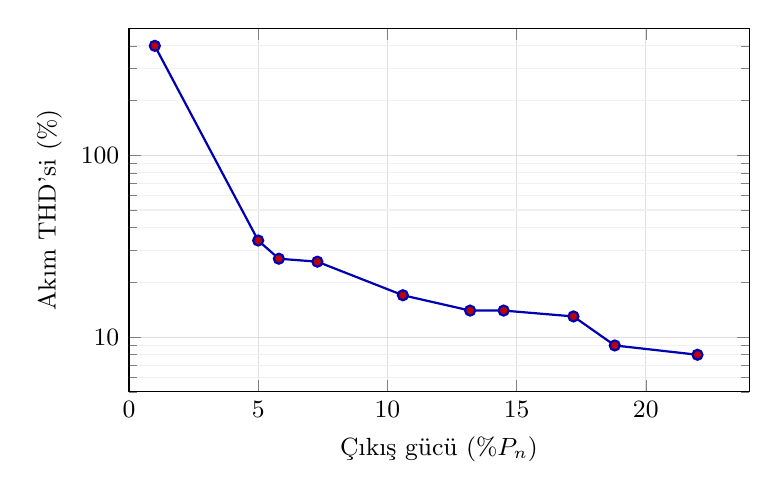
\begin{tikzpicture}
\begin{semilogyaxis}[
  width=0.78\textwidth, height=62mm,
  tick label style={font=\fontsize{9}{10.5}\selectfont}, label style={font=\fontsize{9}{10.5}\selectfont},
  xlabel={Çıkış gücü (\%$P_n$)}, ylabel={Akım THD'si (\%)},
  xmin=0, xmax=24, ymin=5, ymax=500,
  grid=both, grid style={gray!25}, minor grid style={gray!12},
  log basis y=10, log ticks with fixed point, /pgf/number format/use comma,
]
  \addplot[blue!70!black, thick, mark=*, mark size=1.8pt, mark options={fill=red!75!black}] coordinates {
    (1,400) (5,34) (5.8,27) (7.29,26) (10.6,17) (13.2,14) (14.5,14) (17.2,13) (18.8,9) (22,8)};
\end{semilogyaxis}
\end{tikzpicture}

  \caption{Tablo~\ref{tab:ticari-evirici-thd}'deki kaydın grafiği.}
  \label{fig:ticari-evirici-thd}
\end{figure}

Kayıttaki doğrusal olmayan azalma Şekil~\ref{fig:ticari-evirici-thd} üzerinde logaritmik eksende görülmektedir. Akım THD'si anma gücünün \SI{1}{\percent}'inde \SI{400}{\percent} iken \SI{22}{\percent}'sinde \SI{8}{\percent} düzeyine inmektedir. Devreye giriş ve düşük güç test noktaları, anma gücündeki ölçümden ayrı olarak değerlendirilmelidir.

FV profili (Şekil~\ref{fig:fv-calisma-profilleri}, Tablo~\ref{tab:fv-guc-dagilimi}) ile ticari evirici kaydı (Tablo~\ref{tab:ticari-evirici-thd}), düşük güç bölgesinin işletmede sık görüldüğünü ve düşük güçte akım THD'sinin yükseldiğini literatürle birlikte nitel olarak desteklemektedir. Tezdeki verim ve THD bulguları ise deney kayıtlarına ve kalibre edilmiş benzetimlere dayalıdır.

Düşük güçte sürücü, kontrol, anahtarlama ve manyetik elemanların güce zayıf bağlı kayıplarının toplam çıkışa oranı büyümektedir. Şebeke akımının küçük olması, ölü zamanın ve anahtarlama elemanlarının doğrusal olmayan davranışının temel bileşene göre etkisini de artırmaktadır. Saha ve laboratuvar ölçümleri, FV eviricilerde akım dalga biçimi bozulmasının güç seviyesi ve şebeke gerilim kalitesiyle değiştiğini göstermiştir \citep{Kjaer2005,Chicco2009}. Harmonik sınırları bağlantı gücü ve standart kapsamına göre tanımlansa da yalnızca toplam THD değerine bakılması, hangi harmonik bileşenin hangi fiziksel mekanizmadan kaynaklandığını açıklamamaktadır \citep{IEC61000}.

\section{Şebeke Akım Kontrolü ve İleri Besleme Yaklaşımları}

Düşük güç mekanizması tek başına devre düzeyinde çözülemez, çünkü ters akımı kesen her müdahale, akım çevriminin gördüğü denetlenen sistemi de değiştirmektedir. Akım çevriminin temel elemanı olan akım denetleyicisi, şebekeye bağlı bir eviricide referans akım ile ölçülen akım arasındaki hatadan modülasyon gerilimi üretmektedir. Denetleyici yapısı olarak senkron referans çerçevesi, durağan eksen PI kontrolü ve oransal-rezonans (Proportional-Resonant, PR) kontrolü yaygın seçenekler arasındadır. PR denetleyici, temel frekansta yüksek kazanç sağlayarak sinüzoidal referansın kalıcı durum hatasını azaltabilir. Seçili harmoniklerde ek rezonans kolları da kullanılabilir \citep{Teodorescu2006PR,Teodorescu2011}. Akım denetiminin yanında faz kilitlemeli döngü (Phase-Locked Loop, PLL) veya eşdeğer bir eşzamanlama yapısı şebeke faz ve frekans bilgisini üretmekte, tek fazlı sistemlerde ise ortogonal işaret üretimi ve dijital gecikmeler de tasarımın parçası olmaktadır \citep{Blaabjerg2006,Zhou2018}.

LCL filtre, daha küçük toplam endüktansla yüksek frekanslı anahtarlama bileşenlerini zayıflatabilir. Ancak filtre bir rezonans tepesi de oluşturmaktadır. Rezonansı bastırmaya yönelik yöntemlerden pasif sönümleme direnç kaybı doğururken, aktif sönümleme ölçülen akım veya gerilim işaretlerinden sanal empedans etkisi üretmektedir. PR denetleyici ile LCL aktif sönümlemenin birlikte tasarımı, kapalı çevrim kutupları ve kararlılık marjları dikkate alınarak yapılmalıdır \citep{Zhang2014PR}.

Şebeke gerilimi ileri beslemesi ise ortak bağlantı noktasındaki bozucu gerilimin akıma taşınmasını azaltmak için modülasyon girişine ölçülen gerilimden türetilen bir terim eklemektedir. Ancak Lu ve arkadaşları, dijital gecikmenin ileri besleme yolunu LCL rezonansı üzerinde aktif sönümleme veya negatif sönümleme üretebilen dinamik bir elemana dönüştürebildiğini göstermiştir \citep{Lu2016}. Zayıf şebeke koşullarını inceleyen Wang ve arkadaşları da şebeke empedansına bağlı pozitif geri besleme etkisinin faz marjını azaltabileceğini ortaya koymuş ve ileri besleme kanalının frekans seçici biçimde tasarlanması gerektiğini vurgulamıştır \citep{Wang2024}.

Denetleyici ve filtre etkilerinin yanında anahtar ölü zamanı, snubber ve parazitik kapasiteler de komut edilen gerilim ile gerçekleşen faz gerilimi arasında akım yönüne bağlı bir hata oluşturmaktadır. Nitekim Zhang ve Xu, parazitik kapasitelerin anahtarlama kenarlarını sonlu eğimli hâle getirdiğini ve klasik darbe tabanlı ölü zaman kompanzasyonunun özellikle küçük akımlarda yetersiz kalabildiğini deneysel olarak göstermiştir \citep{Zhang2014Deadtime}. Dolayısıyla düşük güç harmonikleri, denetleyici bant genişliğinin yanında modülasyon, anahtar geçişi, akım yönü ve şebeke geriliminin de ortak sonucudur.

Sin\textsuperscript{3} kompanzasyonuna en yakın literatür, kısmi yükte süreksiz iletime giren dönüştürücülerde akım bozulmasının görev oranı kompanzasyonuyla giderilmesidir. Örneğin sürekli iletim için tasarlanan boost PFC dönüştürücüleri düşük yükte şebeke periyodunun bir bölümünde süreksiz iletime girmekte ve klasik akım denetimi giriş akımını bozmaktadır. \citet{DeGusseme2005}, örnek düzeltmesi ile görev oranı ileri beslemesini birleştiren sayısal bir denetimle iki iletim kipinde de düşük harmonikli giriş akımı elde etmiş ve yöntemi \SI{1}{\kilo\watt} prototipte doğrulamıştır. \citet{VanDeSype2005} de görev oranı ileri beslemesinin giriş empedansını dirençsel yaptığını analitik olarak göstermiş ve sıfır geçişi bozulmasını büyük ölçüde gidermiştir. Şebeke eviricisi tarafında ise \citet{Le2019}, sürekli ve süreksiz akım kipinde çalışan tek fazlı bir eviricide süreksiz iletimin yol açtığı doğrusal olmayan davranışı kompanze etmiştir. Bir önceki hesaplama periyodunun görev oranını kullanan kompanzasyon endüktans değerinden bağımsızdır. \SI{4}{\kilo\watt} prototipte daha küçük endüktörle endüktör hacmi \%51 azalmış, 0,1 birim yükteki kayıp ise \%35 düşmüştür. \citet{Wu2013} ise histerezis akım denetimli şebeke eviricisinde sıfır geçişi bozulmasının kaynağını gerçek akım eğiminin referans eğiminden küçük kalmasına bağlamış, kritik faz açısını türetmiş ve çevrimiçi faz öteleme kompanzasyonu önermiştir.

Dört çalışmanın ortak ilkesi, süreksiz iletimin bozduğu akımın görev oranına ya da referansa eklenen bir düzeltme terimiyle giderilmesidir. Tezdeki Sin\textsuperscript{3} terimi ise aynı ilkeyi iki noktada farklı uygulamaktadır. Birincisi, bozulmanın kaynağı diyot doğrultmalı ya da tek anahtarlı bir kat değil, T-tipi nötr kolun bilinçli olarak susturulmasıdır. İkincisi, düzeltme çevrimiçi ölçüm ya da önceki görev oranından değil, şebeke fazından üretilen ve çalışma noktasına kalibre edilen sabit katsayılı bir terimden gelmektedir.

Sin\textsuperscript{3} tabanlı yaklaşımın literatürdeki yerini doğru kurabilmek için üçüncü harmonik enjeksiyonu ile bozucu bastırma amaçlı ileri besleme birbirinden ayrılmalıdır. Klasik üçüncü harmonik enjeksiyonu, faz referanslarına ortak mod bileşeni ekleyerek DA bara kullanım oranını artırmayı veya belirli anahtarlama harmoniklerini düzenlemeyi hedeflemektedir \citep{Holmes2003,Aghdam2013}. Sin\textsuperscript{3} terimi ise nötr anahtar susturma yönteminin oluşturduğu üçüncü harmonik etkisine karşı, ölçülen şebeke işaretinden $\sin^3(\theta)=[3\sin(\theta)-\sin(3\theta)]/4$ özdeşliğiyle üretilen bir şekillendirme bileşenidir. Özdeşliğin Fourier gösterimi terimin matematiksel temelini sağlamaktadır \citep{Oppenheim1997}. Modülasyon girişine eklenen terim, hata sinyalinden türetilen bağımsız bir geri besleme denetleyicisi değil, bir kompanzasyon bileşenidir.

İdeal doğrusal ve doyumsuz modelde dışsal ileri besleme terimi kapalı çevrimin karakteristik paydasını değiştirmeyebilir. Ancak gerçek dönüştürücüde örnekleme, PWM gecikmesi, LCL rezonansı, sınırlayıcılar ve anahtarlamanın çalışma noktasına bağlı doğrusal olmayan davranışı ideal ayrımı sınırlamaktadır. Periyodik çalışma noktaları çevresindeki frekans bağlaşımının incelenmesi gerektiğinde doğrusal zamanla periyodik modeller ve harmonik transfer fonksiyonları (Harmonic Transfer Function, HTF) kullanılabilir \citep{Wereley1991,Liao2022}. Sin\textsuperscript{3} terimi için temel gereksinim, kapalı çevrim aktarımının ve düşük ile anma gücü koşullarındaki etkisinin doğrulanmasıdır.

\section{Literatürün Karşılaştırmalı Değerlendirilmesi}

Makale düzeyindeki çalışmaların yanında konuya yakın doktora tezleri de incelenmiştir. \citet{Kerekes2009}, doktora tezinde transformatörsüz FV eviricilerinde verim kazancının getirdiği kaçak akım sorununu incelemiş ve kaçak akımı standart sınırları içinde tutan topolojileri değerlendirmiştir. \citet{Hartmann2011} ise uçak uygulamaları için üç fazlı PWM doğrultucularda güç yoğunluğu ve verimin birlikte en iyilenmesini ele almış olup çalışması Vienna tipi doğrultucuyu da kapsamaktadır. \citet{Dong2012}, konut ve ticari binalar için DA dağıtım sisteminin merkezindeki çift yönlü AA--DA arayüz dönüştürücüsünü incelemiştir. Dong'un tezinde dengesiz tek fazlı şebeke gücünün DA sistem üzerindeki etkisi çözümlenmiş, iki katlı bir topoloji ve sayısal denetim önerilmiş, ayrıca tam köprüye göre toplam hacmin üç kata kadar azaltılabildiği gösterilmiştir. \citet{Wereley1991} ise doktora tezinde doğrusal zamanla periyodik sistemlerin analizine HTF çerçevesini kazandırmıştır.

Tezdeki üç katkı ekseniyle en yakından ilişkili çalışmalar ise Tablo~\ref{tab:literatur-karsilastirma} üzerinde kullanılan yapı, doğrulama düzeyi, tez açısından kalan sınır ve ilişkili araştırma sorusu bakımından karşılaştırılmıştır. Karşılaştırmanın temel ölçütü, çalışmaların tezdeki araştırma sorularını ne ölçüde kapsadığıdır. Tabloda çalışmalar dört öbekte sıralanmıştır: T-tipi topoloji, hafif yükte süreksiz iletim ve kompanzasyon, akım denetimi ve ileri besleme, işlev paylaşımı ve yeniden yapılandırma.

{\footnotesize
\setlength{\tabcolsep}{3pt}
\begin{longtable}{>{\raggedright\arraybackslash}p{0.18\textwidth} >{\raggedright\arraybackslash}p{0.21\textwidth} >{\raggedright\arraybackslash}p{0.19\textwidth} >{\raggedright\arraybackslash}p{0.28\textwidth} >{\centering\arraybackslash}p{0.05\textwidth}}
\caption{Tezle doğrudan ilişkili çalışmaların karşılaştırmalı sentezi. AS: ilişkili araştırma sorusu.}\label{tab:literatur-karsilastirma}\\
\toprule
\textbf{Çalışma} & \textbf{Yapı ve odak} & \textbf{Doğrulama} & \textbf{Tez açısından kalan sınır} & \textbf{AS} \\
\midrule
\endfirsthead
\caption[]{Tezle doğrudan ilişkili çalışmaların karşılaştırmalı sentezi (devamı).}\\
\toprule
\textbf{Çalışma} & \textbf{Yapı ve odak} & \textbf{Doğrulama} & \textbf{Tez açısından kalan sınır} & \textbf{AS} \\
\midrule
\endhead
\bottomrule
\endfoot
\multicolumn{5}{@{}l}{\textit{T-tipi topoloji}} \\*
\citet{Schweizer2013} & Üç seviyeli T-tipi dönüştürücü (kayıp ve verim) & Analitik kayıp hesabı ve donanım prototipi & Düşük güçte nötr kol ters akımı ve ters akıma bağlı THD ele alınmamıştır. & 1, 2 \\
\citet{Schweizer2013Karsilastirma} & Üç seviyeli topolojilerin iki seviyeli sistemlerle karşılaştırması (çip alanı, harmonik kayıp, pasif hacim) & Karşılaştırmalı analitik değerlendirme & Ölçüt tasarım noktasıdır. Düşük akımda nötr kol akım yolu karşılaştırılmamıştır. & 1 \\
\citet{Wang2020} & \SI{250}{\kilo\watt} SiC T-tipi evirici (güç yoğunluğu ve geçiş kayıpları) & Kayıp modeli ve tam ölçekli prototip & Çalışma çekiş eviricisine ve yüksek güç tasarımına odaklanmıştır. & 1 \\
\citet{Kerekes2009} (doktora tezi) & Transformatörsüz FV eviricileri (kaçak akım ve topoloji seçimi) & Analiz ve modelleme & Verim--kaçak akım ödünleşimi incelenmiştir. Düşük güç verim--THD ödünleşimi kapsam dışıdır. & 2 \\
\midrule
\multicolumn{5}{@{}l}{\textit{Hafif yükte süreksiz iletim ve kompanzasyon}} \\*
\citet{Chen2010} & Senkron alçaltıcı (diyot benzetimi ve sürekli iletim) & Analiz, benzetim ve deney & T-tipi şebeke eviricisinin sıfır durumu ve harmonik sonucu kapsanmamıştır. & 1, 2 \\
\citet{DeGusseme2005} & Boost PFC (sürekli ve süreksiz iletimde sayısal denetim, görev oranı ileri beslemesi) & \SI{1}{\kilo\watt} prototip & Bozulma kaynağı tek anahtarlı PFC katıdır. Şebeke eviricisi ve kararlılık etkisi ele alınmamıştır. & 3 \\
\citet{VanDeSype2005} & Boost PFC (görev oranı ileri beslemesi, giriş empedansı) & Analitik model ve prototip & Sıfır geçişi bozulması hedeflenmiştir. Üçüncü harmonik ağırlıklı alternans içi bozulma kapsanmamıştır. & 3 \\
\citet{Le2019} & Tek fazlı şebeke eviricisi (iki akım kipinde, endüktanstan bağımsız süreksiz iletim kompanzasyonu) & \SI{4}{\kilo\watt}, \SI{100}{\kilo\hertz} prototip & Süreksiz iletim küçük endüktör tasarımından gelmektedir. Nötr anahtar susturma ve T-tipi yapı ele alınmamıştır. & 2, 3 \\
\citet{Wu2013} & Histerezis akım denetiminde sıfır geçişi bozulması & Analiz, benzetim ve deney & Kompanzasyon faz ötelemedir. Anahtarlama kipinin değiştirilmesinden doğan bozulma kapsanmamıştır. & 3 \\
\citet{Zhang2014Deadtime} & Ölü zaman ve parazitik kapasite kompanzasyonu & Darbe modeli ve deney & Nötr anahtar susturma kaynaklı üçüncü harmonik hedeflenmemiştir. & 3 \\
\midrule
\multicolumn{5}{@{}l}{\textit{Akım denetimi ve ileri besleme}} \\*
\citet{Lu2016} & LCL eviricide şebeke gerilimi ileri beslemesi & Frekans alanı analizi ve deney & Sin\textsuperscript{3} tabanlı anlık şekillendirme ve düşük güç ters akımı ele alınmamıştır. & 3 \\
\citet{Wang2024} & Zayıf şebekede filtreli ileri besleme & Empedans modeli ve yarı fiziksel benzetim & Amaç anahtarlama kaynaklı üçüncü harmonik değil, şebeke empedansına uyumdur. & 3 \\
\citet{Dong2012} (doktora tezi) & Çift yönlü tek fazlı AA--DA arayüz dönüştürücüsü (DA dağıtım sistemi) & Analiz, topoloji ve sayısal denetim tasarımı & İki katlı topoloji ve sistem düzeyi denetim incelenmiştir. T-tipi düşük güç anahtarlaması kapsam dışıdır. & 3, 4 \\
\midrule
\multicolumn{5}{@{}l}{\textit{İşlev paylaşımı ve yeniden yapılandırma}} \\*
\citet{Haghbin2013} & Araçta tümleşik şarj (sürücü elemanlarının şarjda kullanımı) & İnceleme ve önerilen yalıtımlı şarj devresi & Çekiş sürücüsü ve motor sargısı üzerine kuruludur. Sabit EDS'de T-tipi ve Vienna işlev paylaşımı ele alınmamıştır. & 4 \\
\citet{Yilmaz2013} & Şarj cihazı topolojileri, güç seviyeleri ve altyapı & İnceleme & Sınıflandırma çalışmasıdır. Ortak yarı iletken tabanlı kip geçişi ayrıntılandırılmamıştır. & 4 \\
\citet{Hartmann2011} (doktora tezi) & Üç fazlı PWM ve Vienna tipi doğrultucular (güç yoğunluğu ve verim) & Karşılaştırmalı tasarım ve en iyileme & Doğrultucu tek işlevlidir. Evirici ve batarya yönetimiyle donanım paylaşımı ele alınmamıştır. & 4 \\
\citet{Momayyezan2016} & Yeniden yapılandırılabilir yüksek gerilim batarya dönüştürücüsü & Beş modüllü ölçekli prototip & Şebekeye bağlı üç seviyeli T-tipi evirici ve düşük güç yöntemiyle bütünleşmemiştir. & 4 \\
\citet{Farakhor2023} & Modüler yeniden yapılandırılabilir BESS ve hücre gücü yönetimi & Optimizasyon, benzetim ve laboratuvar prototipi & T-tipi/Vienna işlev paylaşımı ve şebeke akımı kalitesi hedeflenmemiştir. & 4 \\
\citet{Huang2024} & Anahtar tabanlı modüler yeniden yapılandırma ve dengeleme & Kayıp analizi ve ölçekli deney & İlave modül anahtarları kullanılmıştır. Ortak T-tipi güç katı ele alınmamıştır. & 4 \\
\end{longtable}
}


\section{Araştırma Boşluğu}

Literatür taraması dört ayrı bilgi kümesinin gelişmiş olduğunu göstermiştir. T-tipi dönüştürücüye ilişkin çalışmalar yüksek verim, güç yoğunluğu, anahtarlama geçişleri ve elektromanyetik uyumluluk özelliklerini anma ve tasarım noktasında açıklamaktadır \citep{Schweizer2013,Schweizer2013Karsilastirma,Wang2020,Hizarci2021}. Hafif yük çalışmaları ise ters akımı azaltan süreksiz iletim veya diyot benzetimi ilkelerini ve süreksiz iletimin bozduğu akımın görev oranı ileri beslemesiyle düzeltilmesini incelemektedir \citep{Chen2010,DeGusseme2005,VanDeSype2005,Le2019,Wu2013}. Şebeke eviricilerinde akım denetimi, LCL kararlılığı ve şebeke gerilimi ileri beslemesi de ayrı bir literatür oluşturmaktadır \citep{Lu2016,Wang2024,Zhang2014PR}. Son olarak işlev paylaşımı çalışmaları, eviricinin yarı iletkenlerini şarj kipinde yeniden kullanan tümleşik şarj cihazlarını ve batarya modüllerini farklı çalışma kiplerinde yeniden kullanan EDS mimarilerini geliştirmektedir \citep{Haghbin2013,Yilmaz2013,Momayyezan2016,Farakhor2023,Huang2024}.

Ne var ki kümeler arasındaki bağlantı sınırlıdır. Birincisi, T-tipi eviricinin düşük güçte sıfır durumunu oluşturan nötr kolun senkron alçaltıcı benzeri ters akım mekanizması, aynı müdahalenin verim ve üçüncü harmonik üzerindeki karşıt etkileriyle birlikte yeterince incelenmemiştir. İkincisi, süreksiz iletim bozulmasının kompanzasyonu PFC katları ve küçük endüktörlü şebeke eviricileri için çevrimiçi yöntemlerle geliştirilmiş olsa da T-tipi yapıda bozulma nötr anahtarın bilinçli susturulmasından doğmaktadır. Dolayısıyla şebeke fazından üretilen sabit katsayılı bir Sin\textsuperscript{3} teriminin bozulmayı ne ölçüde giderdiği ve akım çevriminin kararlılığını değiştirip değiştirmediği açık bir sorudur. Üçüncüsü, tümleşik şarj ve yeniden yapılandırılabilir batarya literatüründe işlev paylaşımının mümkün olduğu görülmekle birlikte, T-tipi evirici, Vienna PFC ve aktif batarya yönetimi işlevlerinin aynı yarı iletken yapıda birleştirilmesi düşük güç anahtarlama ve şebeke akımı kalitesi ekseniyle ortak bir tez çerçevesinde incelenmemiştir.

Belirlenen araştırma boşluğu, üç katkıyı tek bir sav altında birleştirmektedir. Sav, T-tipi dönüştürücünün anahtarlama durumlarının düşük güçte ters akımı azaltacak biçimde yeniden düzenlenebileceğini, ortaya çıkan harmonik ödünleşiminin Sin\textsuperscript{3} tabanlı ileri besleme kompanzasyonuyla yönetilebileceğini ve aynı topolojinin yarı iletkenlerinin EDS'nin farklı şarj--deşarj ve dengeleme kiplerinde yeniden görevlendirilebileceğini önermektedir.
